\model{Sierpiński Triangle}

Open \textit{Triangles.java} and run the program.
Then change \java{LEVELS} to 1 and run the program again.
Observe other \java{LEVELS} from 2 to 5.
Adjust the \java{DELAY} in \textit{Drawing.java}, as needed, to see the full drawing.
Then answer the questions below to explore and discuss the source code as a team.

\vspace{1em}
\begin{minipage}[t]{0.41\linewidth}

\begin{center}
\textbf{Drawing (cropped)}
\end{center}

\fbox{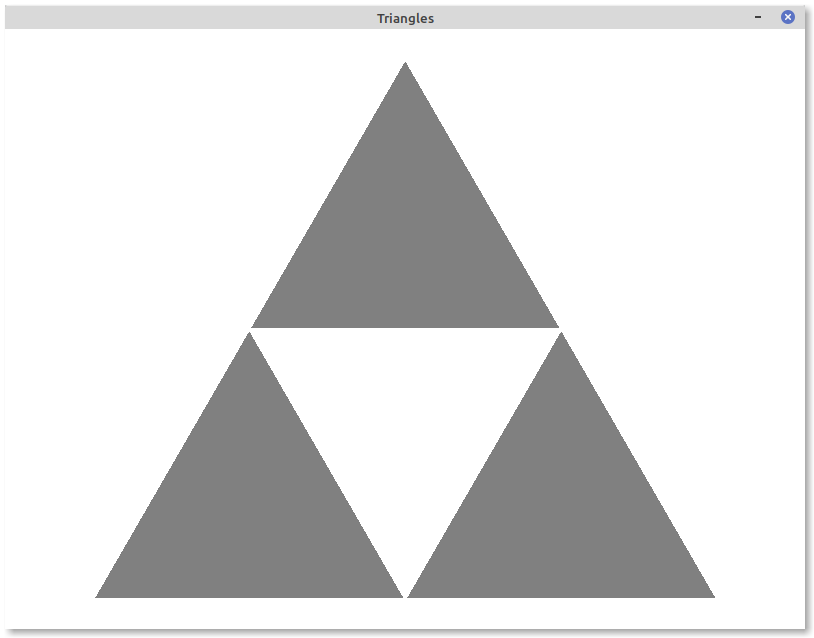
\includegraphics[trim=50 15 50 35,clip,width=\linewidth]{Triangles.png}}

\end{minipage}
\hfill
\begin{minipage}[t]{0.55\linewidth}

\begin{center}
\textbf{Console output}
\end{center}

\footnotesize
\begin{javalst}
Starting tri (88, 570), (400, 30), (712, 570)
    Starting tri (88, 570), (244, 300), (400, 570)
    Finished tri (88, 570), (244, 300), (400, 570)
    Starting tri (244, 300), (400, 30), (556, 300)
    Finished tri (244, 300), (400, 30), (556, 300)
    Starting tri (400, 570), (556, 300), (712, 570)
    Finished tri (400, 570), (556, 300), (712, 570)
Finished tri (88, 570), (400, 30), (712, 570)
\end{javalst}
\end{minipage}


\quest{15 min}


\Q How many times is the \java{tri()} method called\ldots

\begin{multicols}{2}
\begin{enumerate}
\item in the source code\,? \ans{4}
\item when \java{LEVELS = 0}\,? \ans{1}
\item when \java{LEVELS = 1}\,? \ans{4}
\item when \java{LEVELS = 2}\,? \ans{13}
\end{enumerate}
\end{multicols}


\Q Consider the vertices in the drawing above (when \java{LEVELS == 1}).
Using the boxes below, indicate the location of \java{p1}, \java{p2}, \java{p3}, \java{p4}, \java{p5}, and \java{p6}.
\textit{Hint:} see Lines 49--51 and 71--73 of the code.

\setlength{\defaultwidth}{2em}

\begin{quote}
\begin{tabular}{lllll}
         &          & \ans{p2} &          &          \\
         &          &          &          &          \\
         & \ans{p4} &          & \ans{p5} &          \\
         &          &          &          &          \\
\ans{p1} &          & \ans{p6} &          & \ans{p3} \\
\end{tabular}
\end{quote}


\Q When the \java{tri()} method calls itself, what value does it pass for \java{level}?

\begin{answer}[3em]
It increases the current level by one.
\end{answer}


\Q What prevents the recursive process from continuing forever?

\begin{answer}[3em]
The ``base case'' when \java{level == LEVELS}.
The \java{tri()} method starts at \java{0} and counts up.
\end{answer}


\Q When starting the drawing with higher \java{LEVELS}, what do the blue outlines represent?

\begin{answer}
Each blue outline represents a currently active method (i.e., stack frame).
At the end of the method, the blue outline is overwritten with a white outline.
\end{answer}


\Q \label{key3}
Compare the \java{VeeTree} program from \ref{model2.tex} with \java{Triangles}.
In terms of recursion, what do they do in common?
How are they different?

\begin{answer}[6em]
Both programs have a drawing method that calls itself.
They both use \java{level} to know when to stop repeating.
In the case of VeeTree, \java{level} increases to 3.
In the case of Triangles, \java{level} increases to \java{LEVELS}.
Either way, \java{level} makes progress toward its goal.
\end{answer}
